\scanpage{17}
\uline{Cas particuliers}

Supposons que $\forall i\in I$, \deleted{$E_i$ \unsure{est|soit} rare dans $X$.} \inserted{on ait} (si $\Sigma_i^+\ \Sigma_i^-$ sont les deux comp. conn. de $X\setminus\Sigma_i$)

\deleted{Alors on \unsure{trouve} que}
\[
\begin{aligned}
\overline{\Sigma_i^+} &= \Sigma_i^+\cup E_i\\
\overline{\Sigma_i^-} &= \Sigma_i^-\cup E_i\hspace{1.5cm}
% M01: source origin (1172,557); observed triangular point, period interpretation retained as alternative.
\mathpunct{\unsure{\begin{tikzpicture}[x=0.01cm,y=-0.01cm,baseline=(monebase)]
\coordinate (monebase) at (0,6);
\path[use as bounding box] (0,0) rectangle (7,7);
\fill (1,5) -- (3,1) -- (5,0) -- (7,5) -- cycle;
\end{tikzpicture}|.}}
\end{aligned}
\]

Alors je dis qu'on a
\[
\overline{\Sigma_{12}}=\Sigma_{12}
% G01: source origin (947,783); primary literal retraced cup, alternative amalg.
\mathbin{\unsure{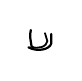
\begin{tikzpicture}[x=0.01cm,y=-0.01cm,baseline=(joinbase)]
\coordinate (joinbase) at (0,29);
\path[use as bounding box] (0,0) rectangle (33,32);
\draw[line width=0.8pt,line cap=round] (4,3) .. controls (2,10) and (4,17) .. (5,24);
\draw[line width=0.65pt,line cap=round] (5,24) .. controls (12,28) and (25,24) .. (25,17) -- (22,7);
\draw[line width=0.8pt,line cap=round] (1,25) .. controls (12,31) and (28,28) .. (30,20) -- (30,8);
\end{tikzpicture}|\amalg}}E_1\cup E_2
\]

% G02: dividing rule; source origin (300,887). The wide fixed rectangle retains its left placement.
\figure{\begin{tikzpicture}[x=0.01cm,y=-0.01cm]
\path[use as bounding box] (0,0) rectangle (1300,25);
\draw[line width=0.3pt,line cap=round] (2,14) .. controls (40,6) and (105,11) .. (145,8) .. controls (183,6) and (222,4) .. (237,8) .. controls (239,9) and (237,12) .. (239,13);
\end{tikzpicture}}

% slanted
\reversemarginpar
\margin{\unsure{introduire|introduisons} la partition $\unsure{\Pi|\pi}_j=\{\deleted{\unsure{\Sigma}}E_j,\Sigma_j^+,\Sigma_j^-\}$}
\normalmarginpar
\deleted{Supposons}

Soit $J\subset I$ tel que $I=J\amalg\{i\}$.

Consid\unsure{e|é}rons la partition
% G03: insertion of Pi_J and bent guide; source origin (1215,1100), fixed rectangle and base-west text anchors.
\begin{tikzpicture}[x=0.01cm,y=-0.01cm,baseline=(pjbase)]
\coordinate (pjbase) at (0,120);
\path[use as bounding box] (0,0) rectangle (175,140);
\begin{scope}[overlay]
\node[anchor=base west,inner sep=0pt,outer sep=0pt] at (10,60) {\inserted{$\Pi_J$}};
\node[anchor=base west,inner sep=0pt,outer sep=0pt] at (100,120) {de};
\draw[line width=0.3pt,line cap=round] (65,111) .. controls (67,91) and (91,90) .. (119,85) .. controls (137,83) and (148,80) .. (151,73);
\end{scope}
\end{tikzpicture}
$X$ \deleted{définie} définie par les $\deleted{\unsure{\Sigma}}E_j$ $(j\in J)$, \unsure{\deleted{et}|et} intersection des partitions
% G04: ternaires Pi_j and its two-branch caret; source origin (950,1350).
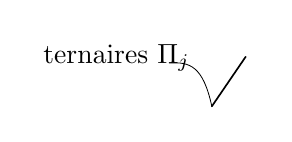
\begin{tikzpicture}[x=0.01cm,y=-0.01cm,baseline=(ternbase)]
\coordinate (ternbase) at (0,100);
\path[use as bounding box] (0,0) rectangle (300,110);
\begin{scope}[overlay]
\node[anchor=base west,inner sep=0pt,outer sep=0pt] at (20,45) {\inserted{ternaires $\Pi_j$}};
\draw[line width=0.3pt,line cap=round] (180,45) .. controls (206,43) and (223,49) .. (234,100);
\draw[line width=0.6pt,line cap=round] (234,100) -- (277,37);
\end{scope}
\end{tikzpicture}
de $X$ $(j\in J)$ définies par les $E_j$ \deleted{$\unsure{E|\in}$} $(j\in J)$
\[
X=E_j\amalg\coprod_{\alpha\in\pi_0(X\setminus E_j)}
% M03: detached short mark near the Sigma head and alpha. Dotless j avoids drawing an additional dot.
% Outer source origin (1145,1624); inner origin is explicitly translated to (1192,1627).
\begin{tikzpicture}[x=0.01cm,y=-0.01cm,baseline=(sigbase)]
\coordinate (sigbase) at (0,70);
\path[use as bounding box] (0,0) rectangle (110,88);
\begin{scope}[overlay]
\node[anchor=base west,inner sep=0pt,outer sep=0pt] at (0,70) {$\Sigma_{\jmath}^{\alpha}$};
\node[anchor=base west,inner sep=0pt,outer sep=0pt] at (47,3) {$\unsure{\begin{tikzpicture}[x=0.01cm,y=-0.01cm,baseline=(mthreebase)]
\coordinate (mthreebase) at (0,0);
\path[use as bounding box] (0,0) rectangle (7,7);
\fill (1,6) -- (0,4) -- (3,0) -- (5,1) -- (6,3) -- cycle;
\end{tikzpicture}}$};
\end{scope}
\end{tikzpicture}
\hspace{3cm}\raisebox{-0.45cm}{$\unsure{\begin{tikzpicture}[x=0.01cm,y=-0.01cm,baseline=(mtwobase)]
% M02a and M02b: source origin (1568,1738); two separate dark specks, with unestablished role and hand.
\coordinate (mtwobase) at (0,0);
\path[use as bounding box] (0,0) rectangle (13,17);
\fill (8,3) -- (10,0) -- (12,3) -- (11,5) -- (8,6) -- cycle;
\fill (1,11) -- (4,10) -- (6,12) -- (3,15) -- (1,14) -- cycle;
\end{tikzpicture}}$}
\]

-- c'est aussi la partition définie par celle de $\displaystyle\bigcup_{j\in J}E_j$ en les $E_j$, et la partition
% G05: raised Pi_J ring and its curved guide; source origin (770,1970).
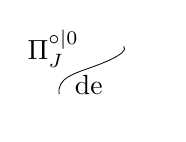
\begin{tikzpicture}[x=0.01cm,y=-0.01cm,baseline=(pjringbase)]
\coordinate (pjringbase) at (0,85);
\path[use as bounding box] (0,0) rectangle (165,110);
\begin{scope}[overlay]
\node[anchor=base west,inner sep=0pt,outer sep=0pt] at (0,40) {\inserted{$\Pi_J^{\unsure{\circ|0}}$}};
\node[anchor=base west,inner sep=0pt,outer sep=0pt] at (60,85) {de};
\draw[line width=0.3pt,line cap=round] (40,84) .. controls (37,64) and (60,58) .. (82,50) .. controls (110,40) and (128,30) .. (122,24);
\end{scope}
\end{tikzpicture}
$\displaystyle X\setminus\mathop{\unsure{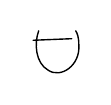
\begin{tikzpicture}[x=0.01cm,y=-0.01cm,baseline=(unionbase)]
% G06: source origin (1115,1975); cup and visible transverse stroke; its mathematical role remains unassigned.
\coordinate (unionbase) at (0,58);
\path[use as bounding box] (0,0) rectangle (70,62);
\draw[line width=0.5pt,line cap=round] (14,4) .. controls (8,20) and (10,45) .. (26,54) .. controls (42,65) and (67,48) .. (65,22) .. controls (65,12) and (63,7) .. (61,4);
\draw[line width=0.5pt,line cap=round] (7,16) -- (56,14);
\end{tikzpicture}}}\limits_{j\in J}E_j$ intersection des partitions binaires $\Pi_{J,j}^{\circ}$
% G07: inserted condition and long hooked guide over induites; source origin (1235,2070).
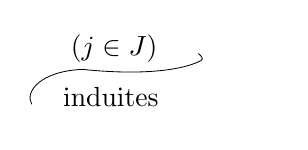
\begin{tikzpicture}[x=0.01cm,y=-0.01cm,baseline=(condbase)]
\coordinate (condbase) at (0,100);
\path[use as bounding box] (0,0) rectangle (320,120);
\begin{scope}[overlay]
\node[anchor=base west,inner sep=0pt,outer sep=0pt] at (55,35) {\inserted{$(j\in J)$}};
\node[anchor=base west,inner sep=0pt,outer sep=0pt] at (45,100) {induites};
\draw[line width=0.3pt,line cap=round] (5,97) .. controls (-4,81) and (17,55) .. (70,53) .. controls (126,59) and (188,58) .. (220,42) .. controls (224,40) and (221,36) .. (217,33);
\end{scope}
\end{tikzpicture}
% G08: inserted U subscript correction and guide; source origin (330,2160).
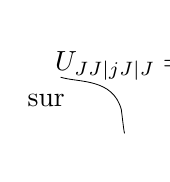
\begin{tikzpicture}[x=0.01cm,y=-0.01cm,baseline=(ubase)]
\coordinate (ubase) at (0,100);
\path[use as bounding box] (0,0) rectangle (145,160);
\begin{scope}[overlay]
\node[anchor=base west,inner sep=0pt,outer sep=0pt] at (0,100) {sur};
\node[anchor=base west,inner sep=0pt,outer sep=0pt] at (35,55) {\inserted{$U_{\unsure{\deleted{J}J|\deleted{j}J|J}}={}$}};
\draw[line width=0.3pt,line cap=round] (42,63) .. controls (65,70) and (108,64) .. (119,104) .. controls (121,120) and (122,130) .. (123,134);
\end{scope}
\end{tikzpicture}
$\displaystyle X\setminus\bigcup_{j\in J}E_j$ par les $\Pi_j$ $(\unsure{g|j}\in J)$. Pour
% archive sheet number: 16
